% !Mode:: "TeX:UTF-8"
\title{实验三 HDFS核心设计 实验报告}
\author{江昱峰 21009200038} 
\documentclass {article}
\usepackage[UTF8]{ctex}
\usepackage{graphicx}
\usepackage{float}
\usepackage{hyperref}
\usepackage{makecell}
\begin{document}
	%\begin{sloppypar}
	\maketitle{}
	\section{背景介绍}
		在我们平常电脑应用上,我们经常会有删除文件的操作。也有时候我们会不小心将文件删除,但这些删除并非永久删除,而是保存在回收站,我们可通过恢复文件将我们删除的文件复原。
		
		HDFS回收机制也是如此,当我们删除文件时,会将删除文件放置在回收站,以备我们误删时恢复。HDFS回收机制默认是关闭的,因此本节实训学习配置并开启垃圾回收机制。
	
	\section{实验目的}
		实践并掌握HDFS核心设计,具体包括以下两部分内容:
		\begin{itemize}
			\item 心跳机制配置;
			\item 垃圾回收机制配置.
		\end{itemize}
	
	\section{实验知识}	
		\noindent 心跳机制简介:
		
		所谓“心跳”是一种形象化描述,指的是持续的按照一定频率在运行,类似于心脏在永无休止的跳动。
			
		心跳机制就是为了证明数据节点还活着,如果一段时间内没有向NameNode发送心跳包信息,就会被Dead状态。并且DataNode从心跳包回复中获取命令信息,然后进行下一步操作,所以从这里可以看出,心跳机制在整个HDFS系统中都有很重要的作用。
	
	\section{实验要求}
		完成HDFS核心设计,具体报考以下两部分任务:
		\begin{itemize}
			\item 配置心跳机制,模拟DataNode节点挂掉,是否在配置时间出现Dead状态。
			\item 配置并开启垃圾回收机制,模拟删除文件并恢复。
		\end{itemize}
	
	\section{实验环境}
		本次实验实验环境为青椒课堂平台的Linux(Centos 7.5)操作系统。
	
	\section{实验步骤与结果分析}
		\subsection{心跳机制配置}
			任务:配置心跳机制文件
			\subsubsection{文件配置}
				\begin{enumerate}
					\item 关闭Hadoop集群。
					\item 进入文件(hdfs-default.xml)所在目录/root/software/hadoop-2.7.7/etc/hadoop/。
					\begin{figure}[H]
						\centering
						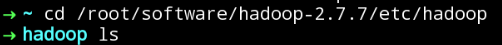
\includegraphics{figures/fig1.png}
					\end{figure}
				
					\item 添加心跳周期为3s。
					\begin{figure}[H]
						\centering
						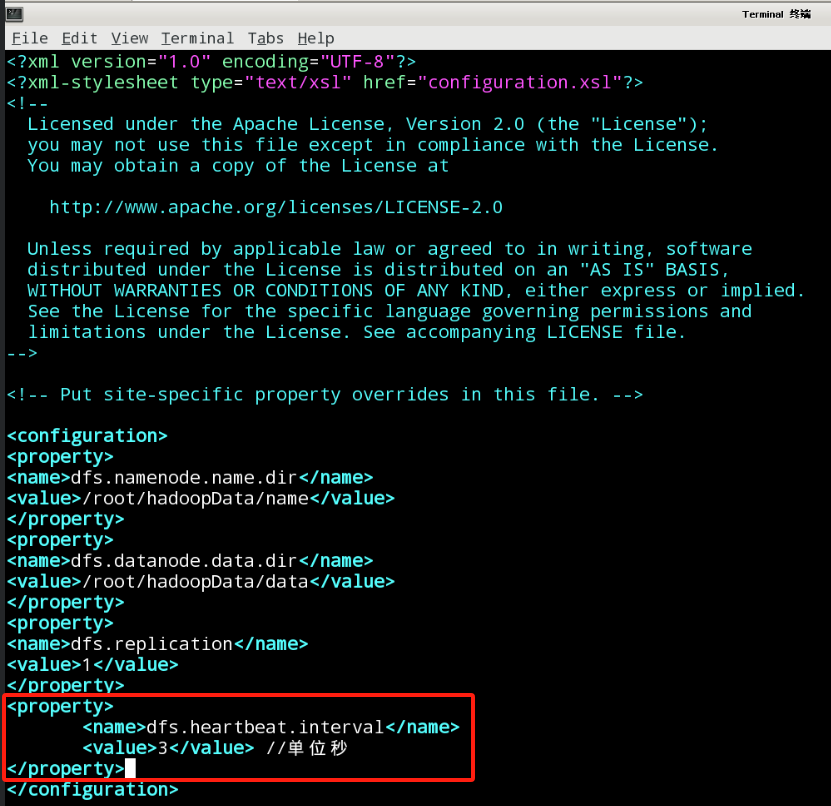
\includegraphics[width=4.5in]{figures/fig2.png}
					\end{figure}
				
					\item 添加心跳检测时长为15s。
					\begin{figure}[H]
						\centering
						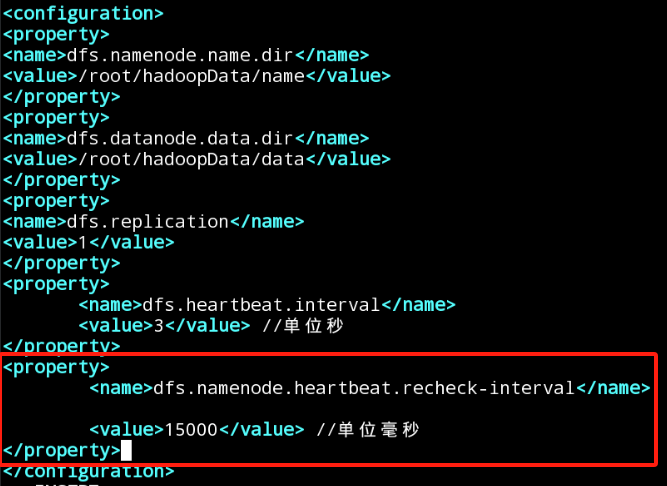
\includegraphics[width=4.5in]{figures/fig3.png}
					\end{figure}
				
					\item 保存配置,重启集群。
					\begin{figure}[H]
						\centering
						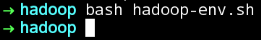
\includegraphics{figures/fig4.png}
					\end{figure}
				\end{enumerate}
		
			\subsubsection{查看DataNode状态}
				\begin{enumerate}
					\item 浏览器访问HDFS Web UI。
					\begin{figure}[H]
						\centering
						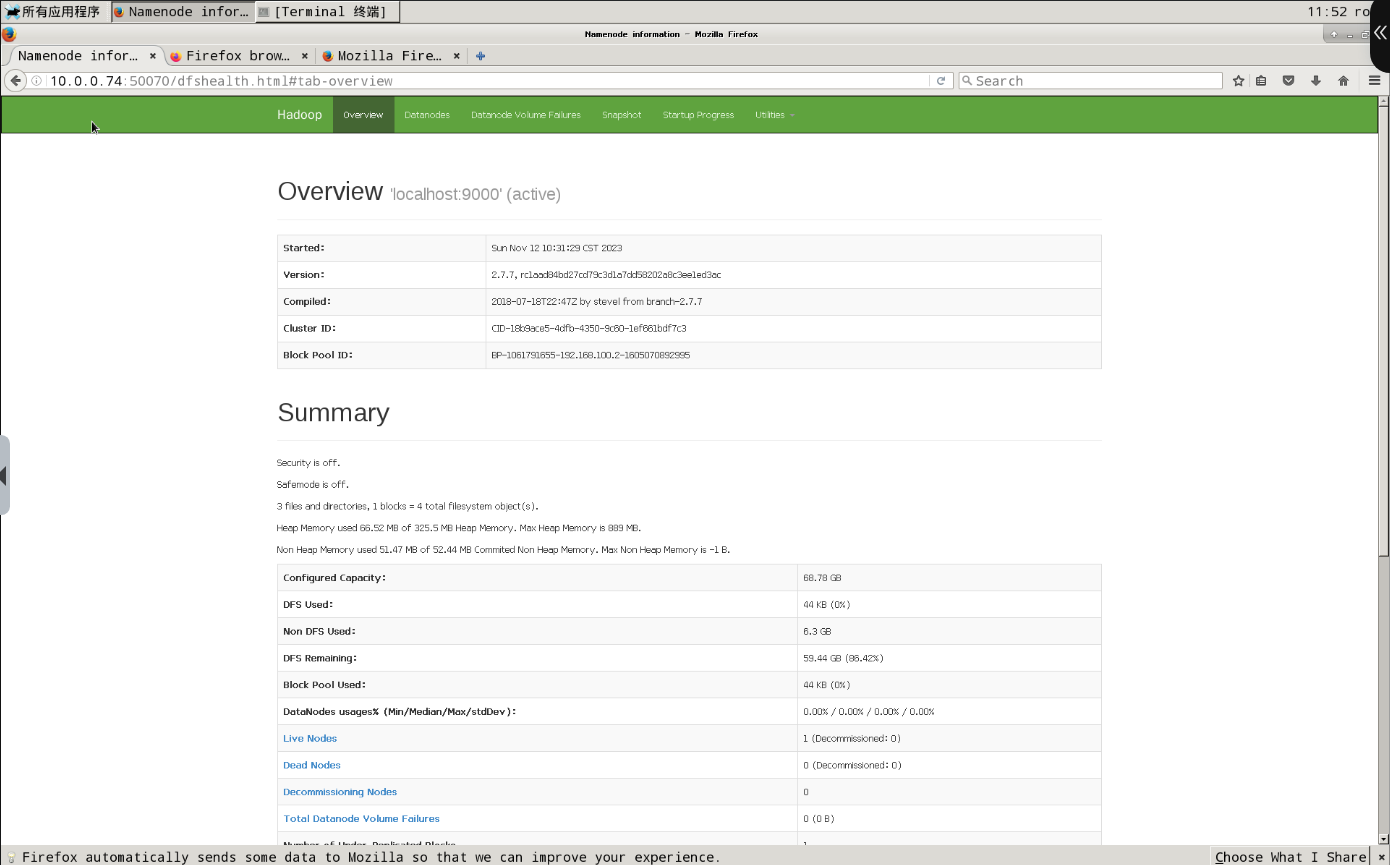
\includegraphics[width=4.5in]{figures/fig5.png}
					\end{figure}
				
					\item 选择DataNode。
					\begin{figure}[H]
						\centering
						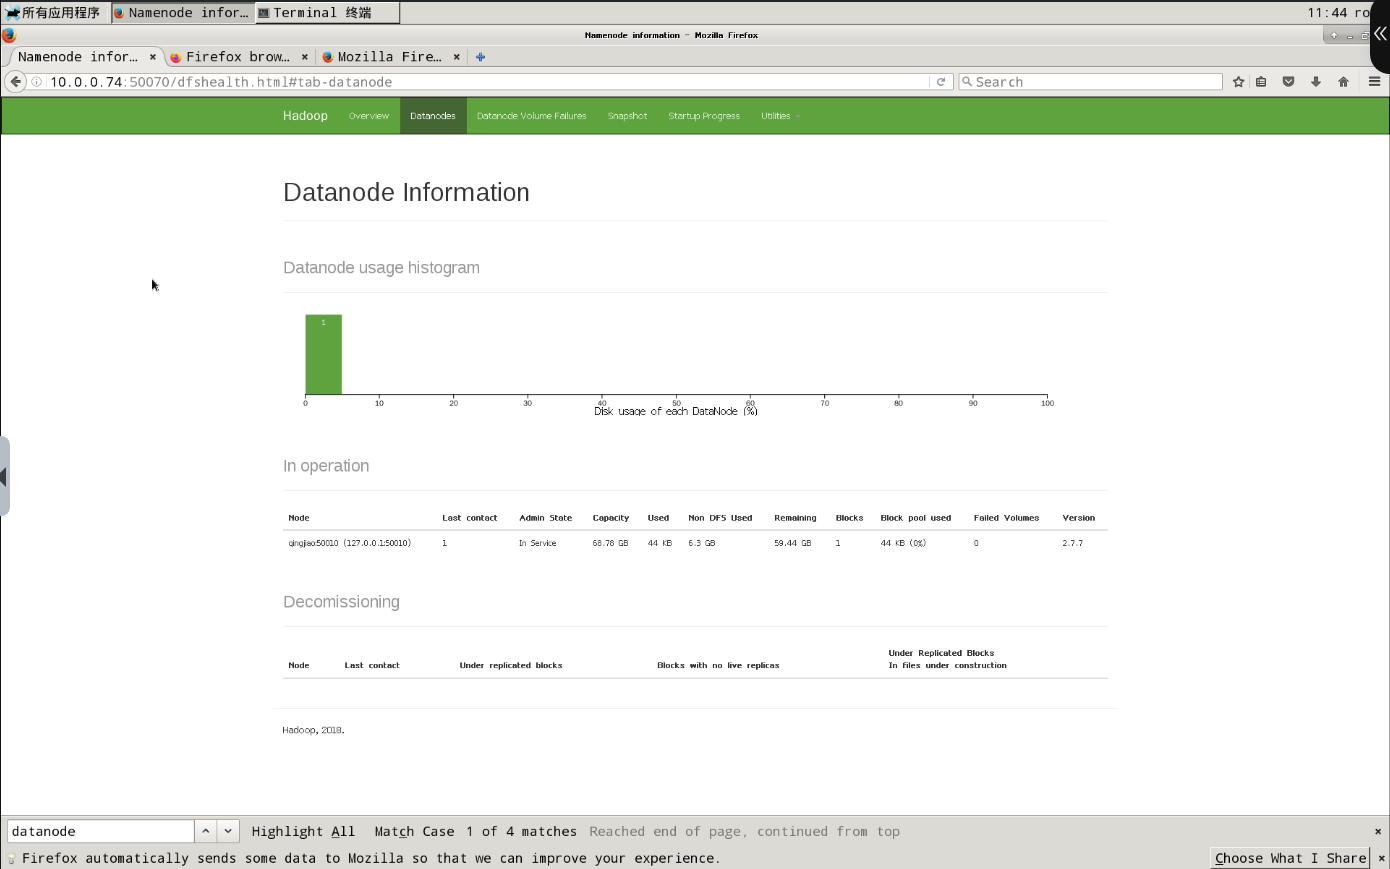
\includegraphics[width=4.5in]{figures/fig6.png}
					\end{figure}
				
					\item 查看Last contact值。通过不断刷新页面发现Last contact值不断增大。
					\begin{figure}[H]
						\centering
						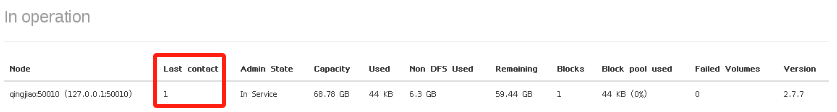
\includegraphics[width=4.5in]{figures/fig7.png}
					\end{figure}
					\begin{figure}[H]
						\centering
						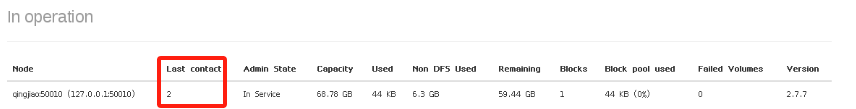
\includegraphics[width=4.5in]{figures/fig8.png}
					\end{figure}
				\end{enumerate}
			
			\subsubsection{模拟DataNode宕机}
				\begin{enumerate}
					\item 通过文件配置,我们计算出宕机时间为1分钟。公式如下:
					
					$Time=2dfs.namenode.heartbeat.recheck-interval+10dfs.heartbeat.interval$
					
					\item 通过jps命令查看进程。
					\begin{figure}[H]
						\centering
						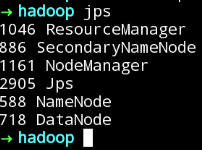
\includegraphics{figures/fig9.png}
					\end{figure}
				
					\item 使用kill命令删除DataNode节点。
					\begin{figure}[H]
						\centering
						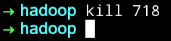
\includegraphics{figures/fig10.png}
					\end{figure}
				
					\item 查看Last contact值。当我们kill掉DataNode进程一分钟左右时间,当我们发现Last contact值报红,显示为Dead装填状态,证明我们配置成功。
					\begin{figure}[H]
						\centering
						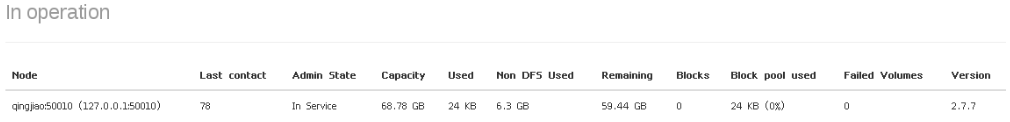
\includegraphics[width=4.5in]{figures/fig10.5.jpg}
					\end{figure}
				\end{enumerate}
			
		\subsection{垃圾回收机制配置}
			\subsubsection{配置垃圾回收机制文件}
				\begin{enumerate}
					\item 关闭集群。
					\item 进入Hadoop安装目录(/root/software/hadoop-2.7.7/etc/hadoop)设置fs.trash.interval值为一天。
					\begin{figure}[H]
						\centering
						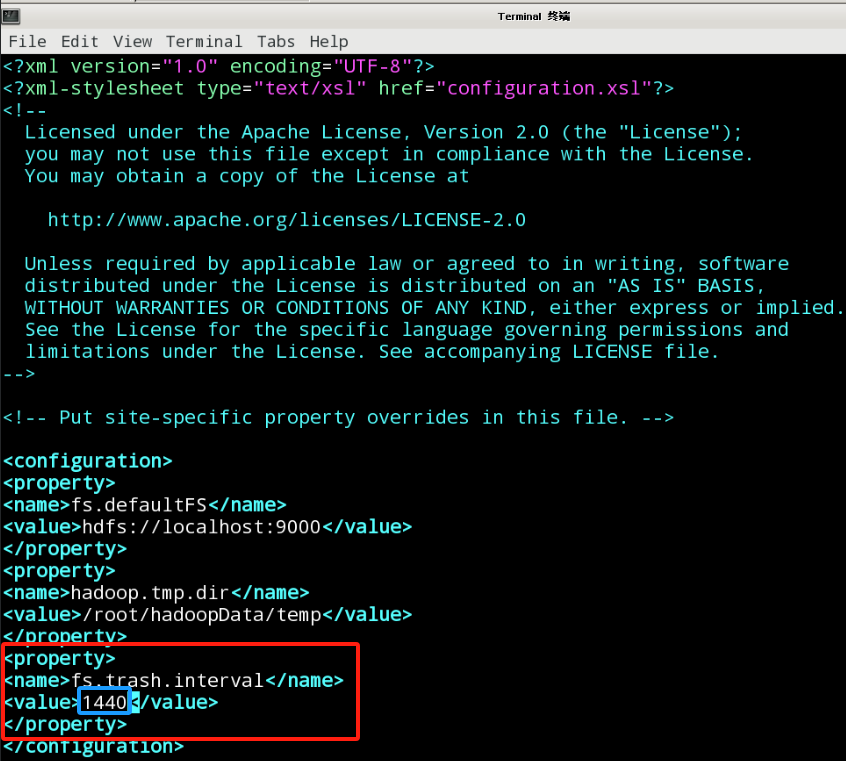
\includegraphics[width=4.5in]{figures/fig12.png}
					\end{figure}
				
					\item 设置fs.trash.checkpoint.interval值与fs.trash.interval相同。
					\begin{figure}[H]
						\centering
						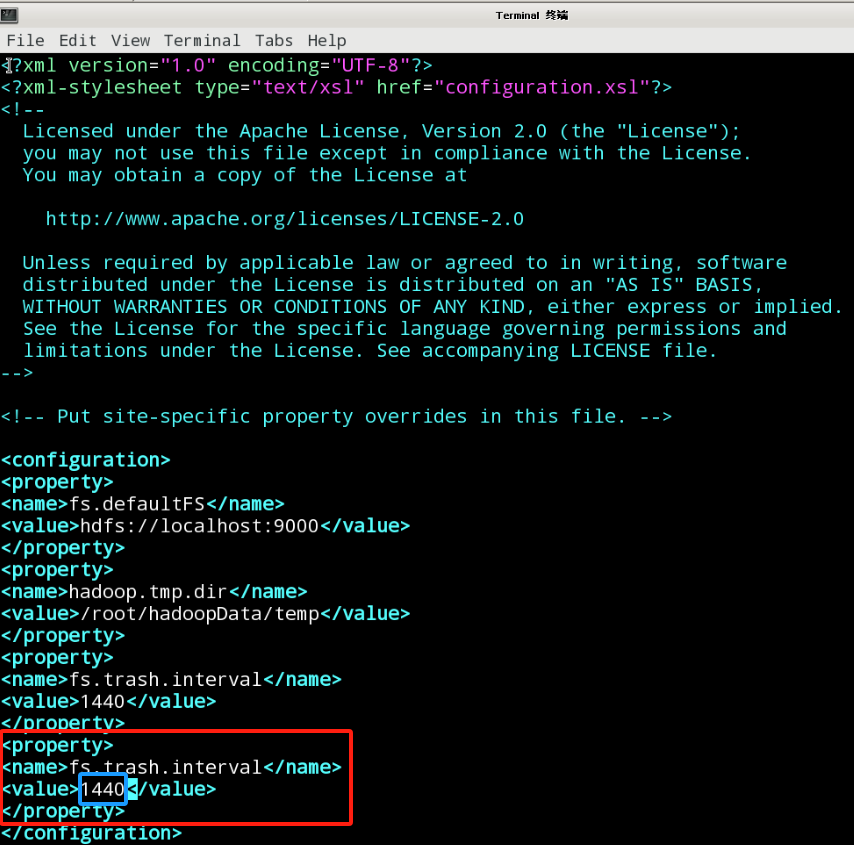
\includegraphics[width=4.5in]{figures/fig13.png}
					\end{figure}
				
					\item 重启集群。
					\begin{figure}[H]
						\centering
						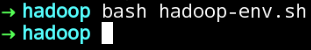
\includegraphics{figures/fig14.png}
					\end{figure}
				\end{enumerate}
			
			\subsubsection{模拟文件删除并恢复}
				\begin{enumerate}
					\item 在/root下创建并编辑文件test.txt。
					编辑内容如下:\\
					core-site.xml \\
					fs.trash.interval \\
					fs.trash.checkpoint.interval
					
					\begin{figure}[H]
						\centering
						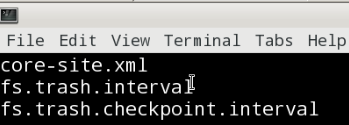
\includegraphics{figures/fig15.png}
					\end{figure}
				
					\item 将文件上传到HDFS根目录。
					\begin{figure}[H]
						\centering
						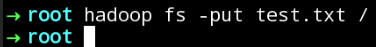
\includegraphics{figures/fig16.png}
					\end{figure}
				
					\item 删除HDFS文件/test.txt。
					\begin{figure}[H]
						\centering
						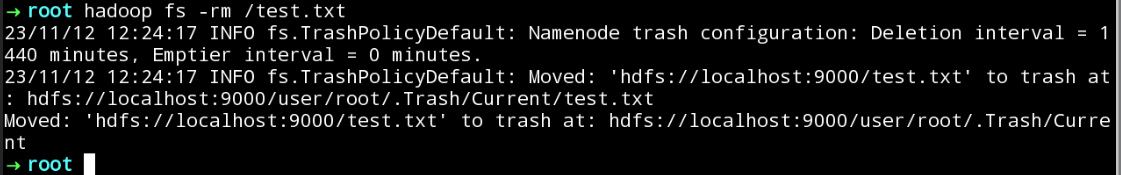
\includegraphics[width=4.5in]{figures/fig17.png}
					\end{figure}
				
					\item 通过执行命令返回信息查看被删除文件所在路径并进入路径查看文件是否存在。
					默认的地址为 “/user/搭建集群的用户名/.Trash/ ”。
					\begin{figure}[H]
						\centering
						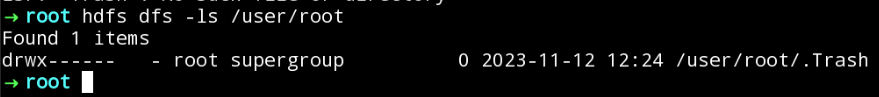
\includegraphics[width=4.5in]{figures/fig18.png}
					\end{figure}
					\begin{figure}[H]
						\centering
						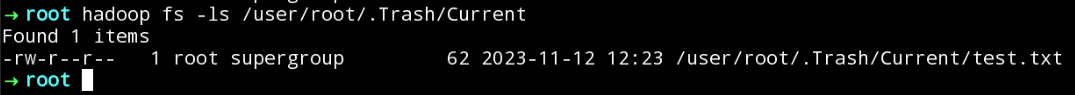
\includegraphics[width=4.5in]{figures/fig19.png}
					\end{figure}
					
					\item 将文件移动到HDFS根目录。
					\begin{figure}[H]
						\centering
						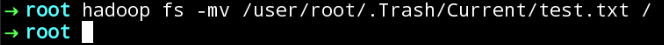
\includegraphics[width=4.5in]{figures/fig20.png}
					\end{figure}
				
					\item 查看文件内容。
					\begin{figure}[H]
						\centering
						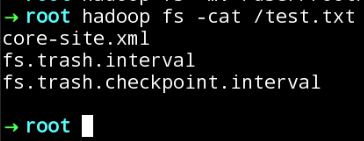
\includegraphics{figures/fig21.png}
					\end{figure}
				\end{enumerate}
			
	\section{结果分析}
		\begin{itemize}
			\item 超过宕机时间后,心跳状态变为Dead。
			\item 类似于Windows操作系统,Hadoop集群中也有指定的回收站用于回收垃圾。
		\end{itemize}
	
	\section{困难解决}
		3.2.3(模拟文件删除并恢复)部分中,执行命令返回的被删除文件所在路径信息与实验平台文档内容提供的路径不完全相同,前者多了一个/Current的子目录。我根据实际情况,判定为文档错误。
	
	\section{心得体会}
		做完本次实验,除了掌握了实验目的部分中所有内容的收获之外,我还有以下几点心得体会:
		\begin{itemize}
			\item 对比分析了心跳机制与TCP协议中三次握手机制等的异同点。
			\item 对比分析了HDFS中的垃圾回收机制与Windows、Linux等操作系统中回收站的异同点。
		\end{itemize}
	
%\end{sloppypar}
\end{document}
\endinput